\documentclass[tikz]{standalone}
\usepackage{tikz}

\usetikzlibrary{positioning}
\usetikzlibrary{fit}
\usetikzlibrary{shapes}
\usetikzlibrary{arrows}

\tikzstyle{X} = [circle,fill=white,draw=black]
% Observed node
\tikzstyle{Y} = [X,fill=gray!25]
\tikzset{>={triangle 45}}

\usetikzlibrary{arrows.meta}
\usepackage{xcolor}

\definecolor{lacamgreen} {RGB} {72, 175, 115}
\definecolor{lacamlilac} {RGB} {107,93,153}
\definecolor{lacamlilac2} {RGB} {93, 109, 152}
\definecolor{lacamlightlilac} {RGB} {174, 166, 201}
\definecolor{lacamdarklilac} {RGB} {51, 10, 102}
\definecolor{lacamgold} {RGB} {255, 87, 0}
\definecolor{lacamdarklilac5} {RGB} {51, 10, 102}
\definecolor{lacamgold5} {RGB} {255, 87, 0}
\definecolor{violet} {RGB} {119, 111, 178}
\definecolor{petroil2} {RGB} {36, 165, 175}
\definecolor{petroil4} {RGB} {30, 132, 149}
\definecolor{petroil6} {RGB} {23, 101, 115}
\definecolor{gold2} {RGB} {255, 130, 0}
\definecolor{gold4} {RGB} {250, 100, 0}
\definecolor{gold6} {RGB} {245, 90, 0}

\newcommand{\highlight}[2][yellow]{\mathchoice%
  {\colorbox{#1}{\strut\textcolor{white}{$\displaystyle{#2}$}}}%
  {\colorbox{#1}{\strut\textcolor{white}{$\textstyle{#2}$}}}%
  {\colorbox{#1}{\strut\textcolor{white}{$\scriptstyle{#2}$}}}%
  {\colorbox{#1}{\strut\textcolor{white}{$\scriptscriptstyle{#2}$}}}}%

\newcommand{\highlighttext}[2][yellow]{{\colorbox{#1}{\strut\textcolor{white}{#2}}}}




\begin{document}

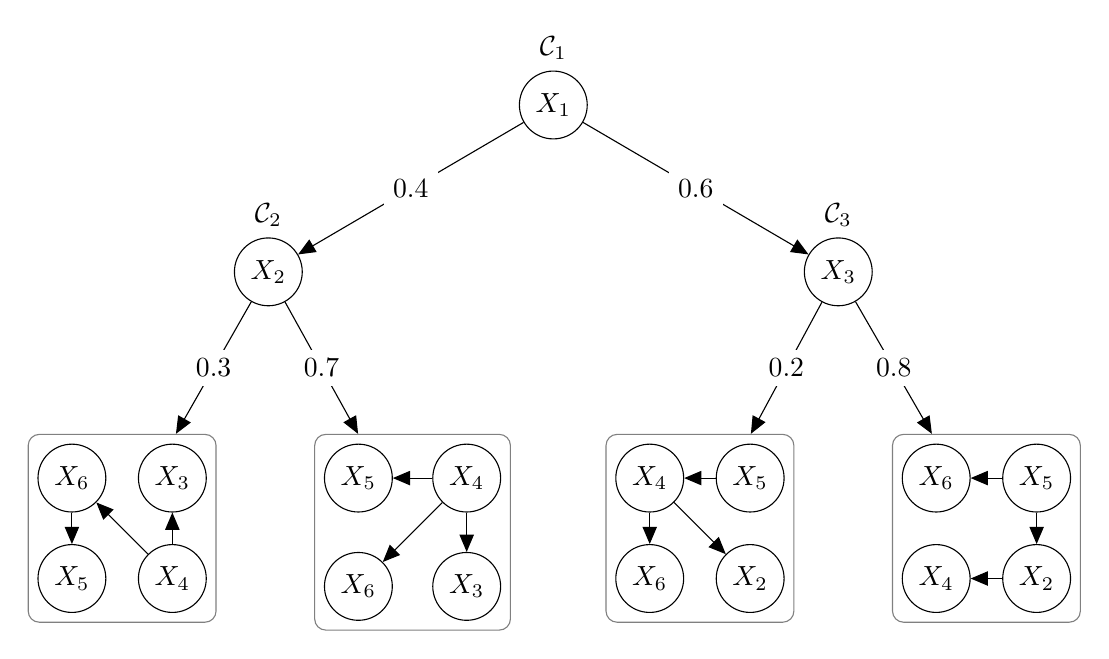
\begin{tikzpicture}
  \node [X] (n1) {$X_1$};    
  \node [X,below left=1.5cm and 3cm of n1] (n2) {$X_2$};    
  \node [X,below right=1.5cm and 3cm of n1] (n3) {$X_3$};    

  \node [above=0.01cm of n1](c1){$\mathcal C_1$};
  \node [above=0.01cm of n2](c2){$\mathcal C_2$};
  \node [above=0.01cm of n3](c3){$\mathcal C_3$};

  \draw [->] (n1) -- (n2) node [midway,fill=white] {0.4};
  \draw [->] (n1) -- (n3) node [midway,fill=white] {0.6};

  \node [X,below right=2cm and 1.9cm of n2] (n7) {$X_4$};
  \node [X,left=0.5cm of n7] (n8) {$X_5$};
  \node [X,below=0.5 of n8] (n9) {$X_6$};
  \node [X,right=0.5 of n9] (n10) {$X_3$};

  \node [draw=gray,rectangle,rounded corners,fit=(n7) (n8) (n9) (n10)] (r1) {};
  \draw [->] (n7) -- (n8) ;
  \draw [->] (n7) -- (n9);
  \draw [->] (n7) -- (n10);
  \draw [->] (n2) -- (r1) node [midway,fill=white] {0.7};
  
  

  
  \node [X,below right=2cm and 1.9cm of n3] (n11) {$X_5$};
  \node [X,left=0.4cm of n11] (n12) {$X_6$};
  \node [X,below=0.4 of n12] (n13) {$X_4$};
  \node [X,right=0.4 of n13] (n14) {$X_2$};
  \node [draw=gray,rectangle,rounded corners,fit=(n11) (n12) (n13)
  (n14)] (r2) {};
  \draw [->] (n3) -- (r2) node [midway,fill=white] {0.8};
  \draw [->] (n11) -- (n12);
  \draw [->] (n14) -- (n13);
  \draw [->] (n11) -- (n14);

   

  \node [X,below left=2cm and .5cm of n3] (n15) {$X_5$};
  \node [X,left=0.4cm of n15] (n16) {$X_4$};
  \node [X,below=0.4 of n16] (n17) {$X_6$};
  \node [X,right=0.4 of n17] (n18) {$X_2$};
  \node [draw=gray,rectangle,rounded corners,fit=(n15) (n16) (n17)
  (n18)] (r3) {};
  \draw [->] (n16) -- (n17);
  \draw [->] (n16) -- (n18);
  \draw [->] (n15) -- (n16);
  \draw [->] (n3) -- (r3) node [midway,fill=white] {0.2};

  \node [X,below left=2cm and .6cm of n2] (n19) {$X_3$};
  \node [X,left=0.4cm of n19] (n20) {$X_6$};
  \node [X,below=0.4 of n20] (n21) {$X_5$};
  \node [X,right=0.4 of n21] (n22) {$X_4$};
  \node [draw=gray,rectangle,rounded corners,fit=(n19) (n20) (n21)
  (n22)] (r4) {};
  \draw [->] (n20) -- (n21);
  \draw [->] (n22) -- (n20);
  \draw [->] (n22) -- (n19);
  \draw [->] (n2) -- (r4) node [midway,fill=white] {0.3};
  


\end{tikzpicture}

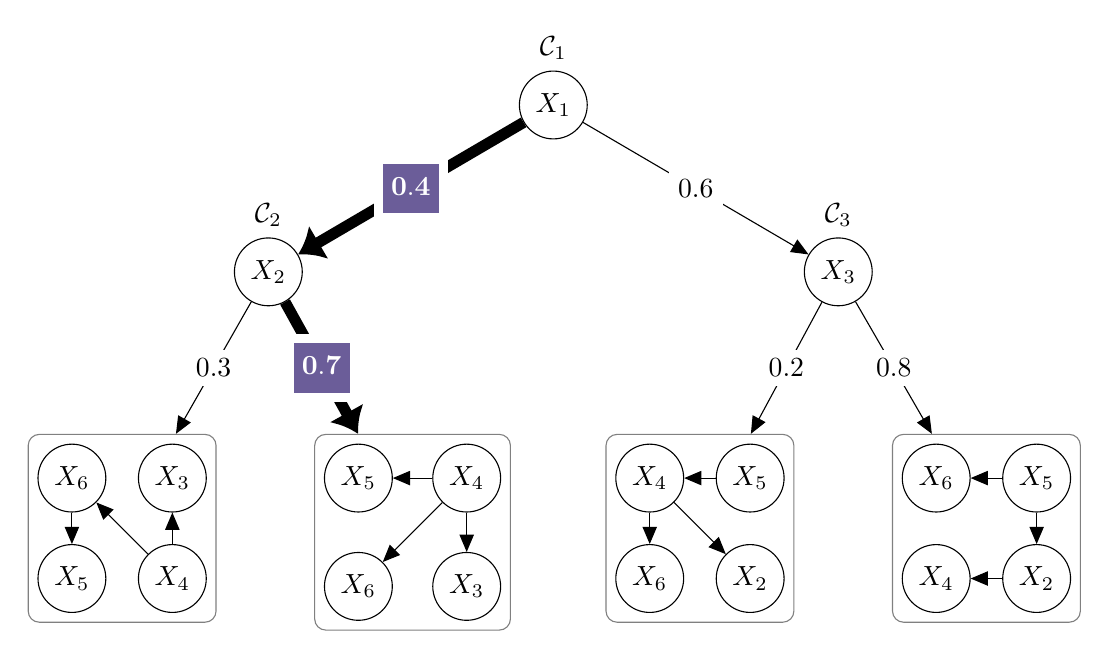
\begin{tikzpicture}
  \node [X] (n1) {$X_1$};    
  \node [X,below left=1.5cm and 3cm of n1] (n2) {$X_2$};    
  \node [X,below right=1.5cm and 3cm of n1] (n3) {$X_3$};    

  \node [above=0.01cm of n1](c1){$\mathcal C_1$};
  \node [above=0.01cm of n2](c2){$\mathcal C_2$};
  \node [above=0.01cm of n3](c3){$\mathcal C_3$};

  \draw [-{Latex[length=3mm,width=5mm]}, line width=4pt] (n1) -- (n2) node [midway,fill=white] {$\highlight[lacamlilac]{\mathbf{0.4}}$};
  \draw [->] (n1) -- (n3) node [midway,fill=white] {0.6};

  \node [X,below right=2cm and 1.9cm of n2] (n7) {$X_4$};
  \node [X,left=0.5cm of n7] (n8) {$X_5$};
  \node [X,below=0.5 of n8] (n9) {$X_6$};
  \node [X,right=0.5 of n9] (n10) {$X_3$};

  \node [draw=gray,rectangle,rounded corners,fit=(n7) (n8) (n9) (n10)] (r1) {};
  \draw [->] (n7) -- (n8) ;
  \draw [->] (n7) -- (n9);
  \draw [->] (n7) -- (n10);
  \draw  [-{Latex[length=3mm,width=5mm]}, line width=4pt] (n2) -- (r1) node [midway,fill=white] {$\highlight[lacamlilac]{\mathbf{0.7}}$};
  
  

  
  \node [X,below right=2cm and 1.9cm of n3] (n11) {$X_5$};
  \node [X,left=0.4cm of n11] (n12) {$X_6$};
  \node [X,below=0.4 of n12] (n13) {$X_4$};
  \node [X,right=0.4 of n13] (n14) {$X_2$};
  \node [draw=gray,rectangle,rounded corners,fit=(n11) (n12) (n13)
  (n14)] (r2) {};
  \draw [->] (n3) -- (r2) node [midway,fill=white] {0.8};
  \draw [->] (n11) -- (n12);
  \draw [->] (n14) -- (n13);
  \draw [->] (n11) -- (n14);

   

  \node [X,below left=2cm and .5cm of n3] (n15) {$X_5$};
  \node [X,left=0.4cm of n15] (n16) {$X_4$};
  \node [X,below=0.4 of n16] (n17) {$X_6$};
  \node [X,right=0.4 of n17] (n18) {$X_2$};
  \node [draw=gray,rectangle,rounded corners,fit=(n15) (n16) (n17)
  (n18)] (r3) {};
  \draw [->] (n16) -- (n17);
  \draw [->] (n16) -- (n18);
  \draw [->] (n15) -- (n16);
  \draw [->] (n3) -- (r3) node [midway,fill=white] {0.2};

  \node [X,below left=2cm and .6cm of n2] (n19) {$X_3$};
  \node [X,left=0.4cm of n19] (n20) {$X_6$};
  \node [X,below=0.4 of n20] (n21) {$X_5$};
  \node [X,right=0.4 of n21] (n22) {$X_4$};
  \node [draw=gray,rectangle,rounded corners,fit=(n19) (n20) (n21)
  (n22)] (r4) {};
  \draw [->] (n20) -- (n21);
  \draw [->] (n22) -- (n20);
  \draw [->] (n22) -- (n19);
  \draw [->] (n2) -- (r4) node [midway,fill=white] {0.3};
  


\end{tikzpicture}


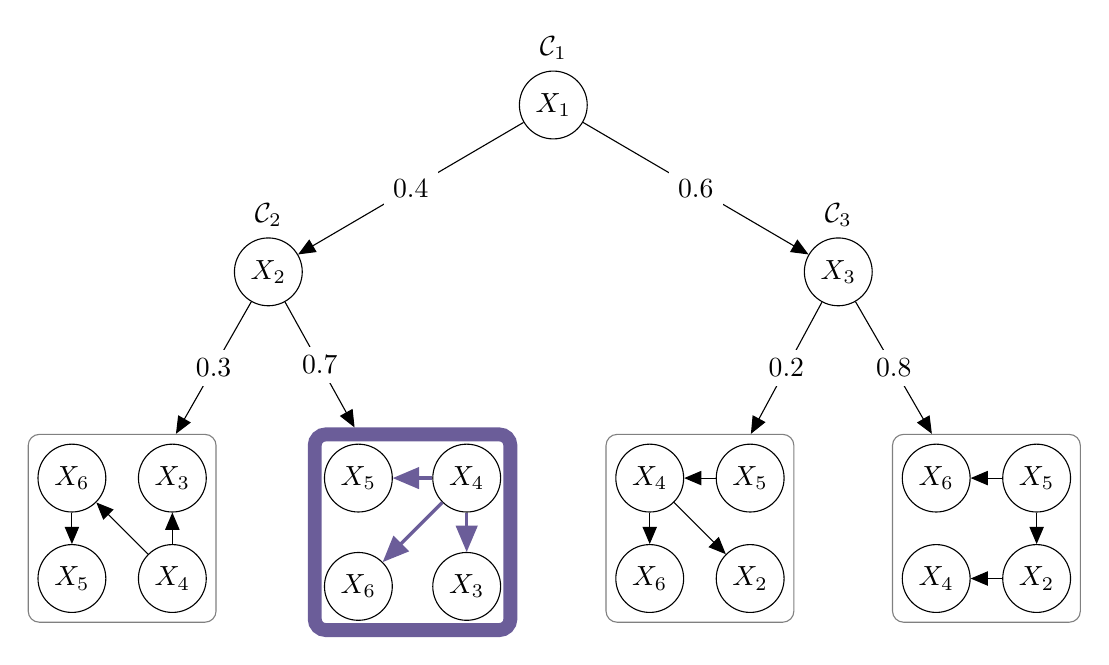
\begin{tikzpicture}
  \node [X] (n1) {$X_1$};    
  \node [X,below left=1.5cm and 3cm of n1] (n2) {$X_2$};    
  \node [X,below right=1.5cm and 3cm of n1] (n3) {$X_3$};    

  \node [above=0.01cm of n1](c1){$\mathcal C_1$};
  \node [above=0.01cm of n2](c2){$\mathcal C_2$};
  \node [above=0.01cm of n3](c3){$\mathcal C_3$};

  \draw [->] (n1) -- (n2) node [midway,fill=white] {0.4};
  \draw [->] (n1) -- (n3) node [midway,fill=white] {0.6};

  \node [X,below right=2cm and 1.9cm of n2] (n7) {$X_4$};
  \node [X,left=0.5cm of n7] (n8) {$X_5$};
  \node [X,below=0.5 of n8] (n9) {$X_6$};
  \node [X,right=0.5 of n9] (n10) {$X_3$};

  \node [draw=lacamlilac,rectangle,line width = 5pt,rounded corners,fit=(n7) (n8) (n9) (n10)] (r1) {};
  \draw [->,color=lacamlilac, line width=1.2pt] (n7) -- (n8) ;
  \draw [->,color=lacamlilac, line width=1.2pt] (n7) -- (n9);
  \draw [->,color=lacamlilac, line width=1.2pt] (n7) -- (n10);
  \draw [->] (n2) -- (r1) node [midway,fill=white] {0.7};
  
  

  
  \node [X,below right=2cm and 1.9cm of n3] (n11) {$X_5$};
  \node [X,left=0.4cm of n11] (n12) {$X_6$};
  \node [X,below=0.4 of n12] (n13) {$X_4$};
  \node [X,right=0.4 of n13] (n14) {$X_2$};
  \node [draw=gray,rectangle,rounded corners,fit=(n11) (n12) (n13)
  (n14)] (r2) {};
  \draw [->] (n3) -- (r2) node [midway,fill=white] {0.8};
  \draw [->] (n11) -- (n12);
  \draw [->] (n14) -- (n13);
  \draw [->] (n11) -- (n14);

   

  \node [X,below left=2cm and .5cm of n3] (n15) {$X_5$};
  \node [X,left=0.4cm of n15] (n16) {$X_4$};
  \node [X,below=0.4 of n16] (n17) {$X_6$};
  \node [X,right=0.4 of n17] (n18) {$X_2$};
  \node [draw=gray,rectangle, rounded corners,fit=(n15) (n16) (n17)
  (n18)] (r3) {};
  \draw [->] (n16) -- (n17);
  \draw [->] (n16) -- (n18);
  \draw [->] (n15) -- (n16);
  \draw [->] (n3) -- (r3) node [midway,fill=white] {0.2};

  \node [X,below left=2cm and .6cm of n2] (n19) {$X_3$};
  \node [X,left=0.4cm of n19] (n20) {$X_6$};
  \node [X,below=0.4 of n20] (n21) {$X_5$};
  \node [X,right=0.4 of n21] (n22) {$X_4$};
  \node [draw=gray,rectangle,rounded corners,fit=(n19) (n20) (n21)
  (n22)] (r4) {};
  \draw [->] (n20) -- (n21);
  \draw [->] (n22) -- (n20);
  \draw [->] (n22) -- (n19);
  \draw [->] (n2) -- (r4) node [midway,fill=white] {0.3};
  


\end{tikzpicture}

\end{document}

%%% Local Variables:
%%% mode: latex
%%% TeX-master: t
%%% End:
